\documentclass[conference]{IEEEtran}

% ── Packages ────────────────────────────────────────────────────────────
\usepackage{graphicx}
\usepackage{amsmath}
\usepackage{booktabs}
\usepackage{hyperref}
\usepackage{cleveref}
\usepackage{subcaption}

\hypersetup{
    colorlinks=true,
    linkcolor=blue,
    citecolor=blue,
    urlcolor=blue,
}

% ── Title ───────────────────────────────────────────────────────────────
\title{Infant Cry Classification Using Classical and Deep Machine Learning:\\
       A Phased Study}

\author{
  \IEEEauthorblockN{Belal Raza}
  \IEEEauthorblockA{Department of Computer Science\\
  Email: belal.raza@example.ac.uk}
}

\begin{document}
\maketitle

% ======================================================================
% ABSTRACT
% ======================================================================
\begin{abstract}
Automatic classification of infant cries can assist caregivers and
clinicians in identifying the cause of neonatal distress.  We address
this problem on the Donate-a-Cry corpus, which contains 457~recordings
spanning five classes: hunger, belly pain, burping, discomfort, and
tiredness.  In this first phase we extract Mel-frequency cepstral
coefficients and spectral descriptors, then evaluate Gaussian Mixture
Model and Support Vector Machine baselines alongside an exploratory
Hidden Markov Model.  Preliminary results indicate that discriminative
models cope better with the severe class imbalance (47.8:1) present in
the dataset.  Phase~2 will introduce deep learning architectures
operating on Mel-spectrogram representations, and Phase~3 will fuse both
paradigms into a hybrid ensemble.
\end{abstract}

% ======================================================================
% 1  INTRODUCTION
% ======================================================================
\section{Introduction}
\label{sec:intro}

Crying is the earliest and most instinctive channel through which
neonates communicate physiological needs.  In clinical neonatal care
units, nurses must simultaneously monitor multiple infants and make rapid
judgements about the cause of each cry episode.  Consumer baby monitors
and smart-nursery devices face a similar challenge: translating raw audio
into actionable information for sleep-deprived caregivers.  An accurate,
real-time cry classifier could reduce response latency, prevent
unnecessary escalation, and support developmental screening in
under-resourced settings~\cite{dunstan2006}.

Several factors make infant cry classification a difficult pattern
recognition problem.  First, inter-class acoustic variability is small:
a hunger cry and a discomfort cry may share fundamental frequency,
harmonic structure, and temporal envelope, differing only in subtle
spectral nuances.  Second, publicly available labelled corpora are
small---the Donate-a-Cry dataset used here contains only 457~clips, with
extreme class imbalance (382~hunger samples versus 8~burping samples).
Third, recordings are captured on consumer-grade devices with variable
background noise, reverberation, and microphone characteristics, which
inject nuisance variation that can overwhelm the discriminative signal.

We adopt a phased study design.  In Phase~1 (this report) we establish
an interpretable classical machine-learning baseline: hand-crafted
acoustic features processed by a Gaussian Mixture Model (GMM), a Support
Vector Machine (SVM), and an exploratory Hidden Markov Model (HMM).
Classical models are fast to train, require no GPU resources, and expose
which acoustic dimensions drive each classification decision---properties
that are important for trust in safety-critical applications.  In
Phase~2 we will train deep learning models (CNN, BiLSTM, attention
mechanisms) on Mel-spectrogram inputs.  Phase~3 will fuse the classical
and deep pipelines into a hybrid ensemble and perform ablation studies.

The remainder of this report is organised as follows.
\Cref{sec:related} reviews relevant literature.
\Cref{sec:dataset} describes the corpus and our preprocessing pipeline.
\Cref{sec:features} details the feature extraction process.
\Cref{sec:models} presents the three classical models evaluated in
Phase~1.  \Cref{sec:results} reports preliminary results and discusses
which classes prove hardest to separate.  Sections covering deep
learning (Phase~2) and the hybrid architecture (Phase~3) will be added
to subsequent versions of this paper as those phases complete.

% ======================================================================
% 2  RELATED WORK
% ======================================================================
\section{Related Work}
\label{sec:related}

% ----------------------------------------------------------------------
\subsection{Classical Approaches to Audio Classification}
\label{sec:related_classical}

Mel-frequency cepstral coefficients (MFCCs) have been the dominant
feature representation in speech and audio classification since their
introduction by Davis and Mermelstein~\cite{davis1980mfcc}.  MFCCs
approximate the human auditory system's frequency resolution via a
Mel-scaled filter bank followed by a discrete cosine transform, yielding
a compact spectral envelope descriptor.

Gaussian Mixture Models became the standard generative classifier in
speaker verification and audio event detection.  Reynolds
\textit{et~al.}~\cite{reynolds2000speaker} demonstrated that
class-conditional densities in MFCC space are well approximated by
mixtures of diagonal-covariance Gaussians, enabling efficient
log-likelihood scoring.  Support Vector Machines offer a complementary
discriminative approach; Chang and Lin's widely-used LIBSVM
library~\cite{chang2011libsvm} showed that RBF-kernel SVMs with proper
regularisation achieve competitive accuracy on moderate-dimensional audio
features.  Hidden Markov Models extend the generative framework by
modelling the temporal sequence of feature frames as a Markov chain of
hidden states, each emitting observations from a Gaussian; Rabiner's
tutorial~\cite{rabiner1989hmm} remains the canonical reference for this
family of models.

% ----------------------------------------------------------------------
\subsection{Infant Cry Recognition}
\label{sec:related_cry}

Ji \textit{et~al.}~\cite{ji2021review} provide a comprehensive survey
of infant cry analysis covering acoustic features, classical classifiers,
and emerging deep-learning methods.  They note that MFCC-based systems
paired with GMMs or SVMs remain competitive on small corpora,
particularly when class imbalance is addressed through data augmentation
or cost-sensitive learning.  Chang and Li~\cite{chang2017infant}
demonstrated early success with deep convolutional networks on
spectrogram representations of infant cries, achieving improvements over
hand-crafted feature baselines on a proprietary hospital dataset.
Lahmiri and Bhatt~\cite{lahmiri2022infant} compared several classical
learners on the Donate-a-Cry corpus and found that ensemble methods and
SVMs outperformed single generative models when combined with careful
feature selection.

% ----------------------------------------------------------------------
\subsection{Deep Learning Approaches}
\label{sec:related_dl}

Large-scale audio classification has been transformed by convolutional
neural networks applied directly to Mel-spectrogram images.  Hershey
\textit{et~al.}~\cite{hershey2017cnn} showed that deep CNN
architectures trained on AudioSet achieve strong generalisation across
diverse sound categories.  Recurrent and attention-based architectures
further exploit temporal structure.  A detailed review of these methods
and their application to infant cry data will be presented in Phase~2 of
this study.

% ======================================================================
% 3  DATASET AND PREPROCESSING
% ======================================================================
\section{Dataset and Preprocessing}
\label{sec:dataset}

% ----------------------------------------------------------------------
\subsection{Donate-a-Cry Corpus}
\label{sec:corpus}

We use the Donate-a-Cry corpus, a publicly available collection of
crowd-sourced infant cry recordings.  The dataset contains
457~recordings distributed across five classes with severe imbalance:
\textit{hunger} accounts for 83.6\% of the data, while \textit{burping}
comprises only 1.7\%.  \Cref{tab:class_dist} summarises the class
distribution.  All recordings are single-channel WAV files captured at a
native sampling rate of 8\,000\,Hz on consumer-grade devices.

\begin{table}[t]
  \centering
  \caption{Class distribution in the Donate-a-Cry corpus.}
  \label{tab:class_dist}
  \begin{tabular}{lrrr}
    \toprule
    \textbf{Class} & \textbf{Samples} & \textbf{\%} & \textbf{Mean Duration (s)} \\
    \midrule
    Hunger     & 382 & 83.6 & 6.95 \\
    Discomfort &  27 &  5.9 & 6.88 \\
    Tiredness  &  24 &  5.3 & 6.84 \\
    Belly pain &  16 &  3.5 & 6.90 \\
    Burping    &   8 &  1.7 & 6.79 \\
    \midrule
    \textbf{Total} & \textbf{457} & \textbf{100} & \textbf{6.92} \\
    \bottomrule
  \end{tabular}
\end{table}

% ----------------------------------------------------------------------
\subsection{Preprocessing Pipeline}
\label{sec:preprocess}

Our preprocessing pipeline applies three stages:

\begin{enumerate}
  \item \textbf{Resampling.}  All clips are loaded at their native
        8\,000\,Hz sampling rate.  Exploratory analysis confirmed that
        every file in the corpus shares this rate, so no resampling is
        required.

  \item \textbf{Padding and truncation.}  Each waveform is normalised to
        a fixed duration of 7\,seconds (56\,000~samples).  Clips shorter
        than 7\,s are zero-padded; clips longer than 7\,s are truncated.
        Analysis showed that 54.7\% of clips require padding and 5.5\%
        require truncation, with durations ranging from 6.52\,s to
        7.06\,s.

  \item \textbf{Data augmentation.}  To mitigate the extreme class
        imbalance, we augment minority classes (all classes except
        \textit{hunger}) to a minimum target of 80~samples per class
        using five transformations: pitch shifting ($\pm 1$, $\pm 2$
        semitones), time stretching ($0.9\times$, $1.1\times$), additive
        white noise (SNR~$\approx$~25--30\,dB), temporal shifting
        ($\pm 0.5$\,s), and a composite perturbation (pitch~$+1$ semitone
        combined with noise).  Up to 10~augmented variants are generated
        per original clip.
\end{enumerate}

Quality checks confirmed zero silent files (minimum RMS energy =
0.00104) and zero corrupted files across the full corpus.

% ======================================================================
% 4  FEATURE EXTRACTION
% ======================================================================
\section{Feature Extraction}
\label{sec:features}

We extract a 246-dimensional feature vector per clip, comprising three
blocks: MFCC statistics, delta and delta-delta statistics, and spectral
descriptors.

\subsection{Mel-Frequency Cepstral Coefficients}

We compute $K = 40$ MFCCs per frame using an FFT window of 512~samples
($\approx$\,64\,ms at 8\,kHz) and a hop length of 160~samples
($\approx$\,20\,ms).  The $n$-th cepstral coefficient is obtained from
the log-Mel filter bank energies $S_k$ via the type-II discrete cosine
transform:

\begin{equation}
  c_n = \sum_{k=1}^{K} \log S_k \,
        \cos\!\left[n\!\left(k - \tfrac{1}{2}\right)\frac{\pi}{K}\right],
        \quad n = 0, 1, \dots, K{-}1.
  \label{eq:mfcc}
\end{equation}

\noindent
Each of the 40~MFCC time series is summarised by its mean and standard
deviation across all frames, yielding $40 \times 2 = 80$ features.  The
same summary statistics are applied to the first- and second-order
temporal difference (delta and delta-delta) coefficients, contributing
an additional $2 \times 80 = 160$ features.

\subsection{Spectral Descriptors}

Six complementary descriptors capture acoustic properties not fully
encoded by MFCCs:

\begin{itemize}
  \item \textbf{Zero-crossing rate (ZCR)} --- a proxy for the
        noisiness and high-frequency content of the signal.
  \item \textbf{Spectral centroid} --- the ``centre of mass'' of the
        spectrum, correlating with perceived brightness.
  \item \textbf{Spectral roll-off} --- the frequency below which a
        specified percentage (85\%) of spectral energy is concentrated.
  \item \textbf{Spectral bandwidth} --- the second central moment of
        the spectrum, measuring spectral spread.
  \item \textbf{RMS energy} --- the root-mean-square amplitude,
        indicating overall loudness.
  \item \textbf{Spectral flatness} --- the ratio of geometric to
        arithmetic mean of the power spectrum, distinguishing tonal from
        noise-like signals.
\end{itemize}

\noindent
Each descriptor contributes one scalar value (frame-level mean), for a
total of 6~features.  Combined with the 240~MFCC-based features, the
full vector has dimensionality $240 + 6 = 246$.

\Cref{fig:mfcc_boxplot} shows the distribution of the top-10 MFCC
features by inter-class variance; MFCC-0 (related to overall spectral
energy) provides the strongest class separation.

\begin{figure}[t]
  \centering
  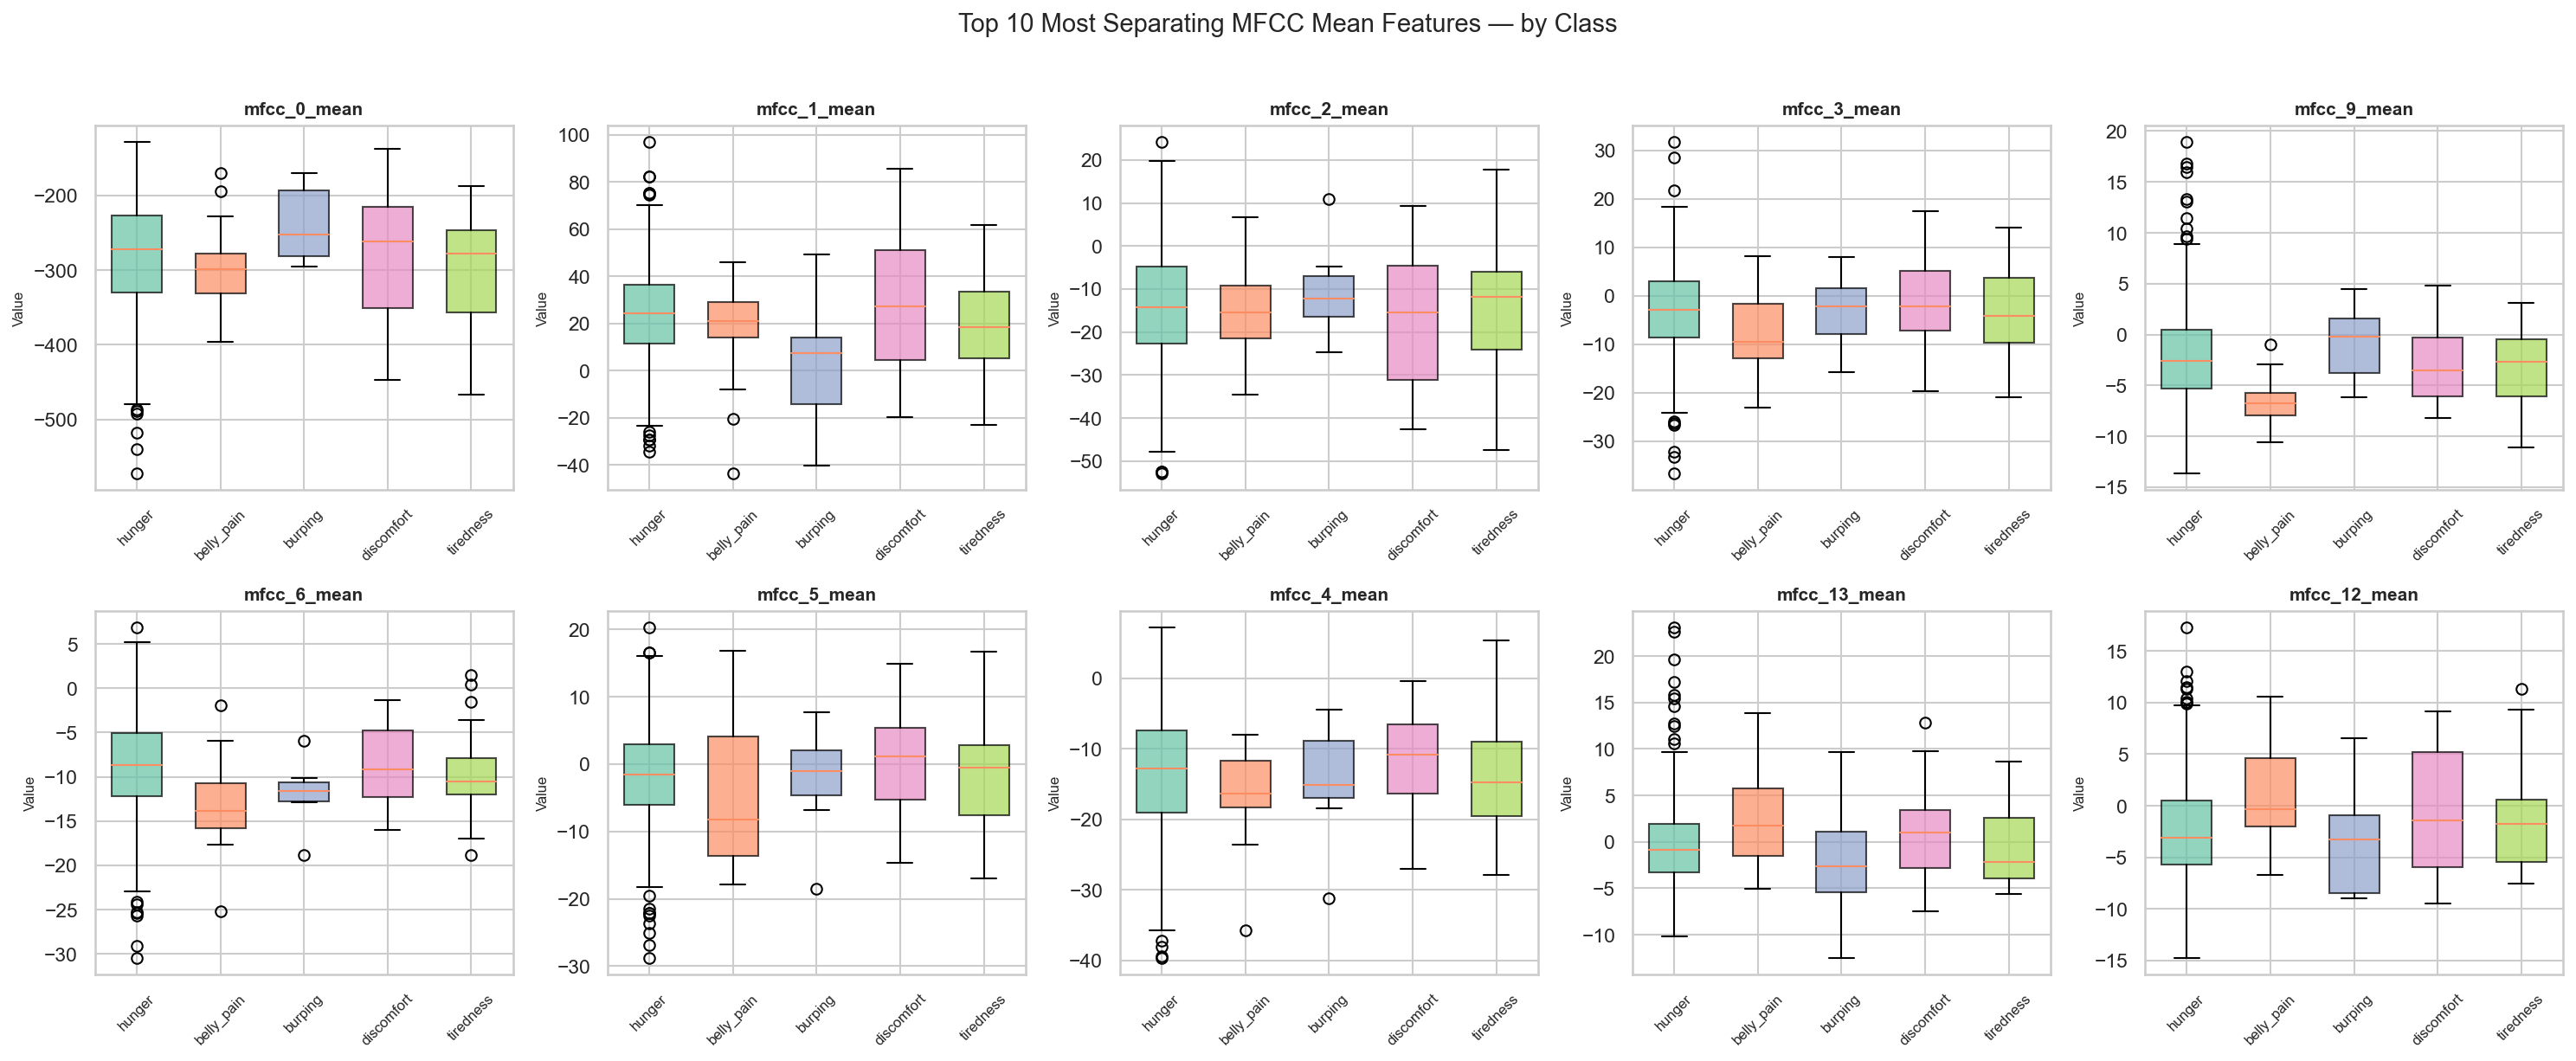
\includegraphics[width=\columnwidth]{../results/plots/mfcc_top10_boxplots.png}
  \caption{Boxplots of the ten MFCC features with highest inter-class
           variance.  MFCC-0 achieves an inter-class variance of 649.4,
           substantially exceeding all other coefficients.}
  \label{fig:mfcc_boxplot}
\end{figure}

% ======================================================================
% 5  CLASSICAL ML MODELS (PHASE 1)
% ======================================================================
\section{Classical ML Models (Phase~1)}
\label{sec:models}

% ----------------------------------------------------------------------
\subsection{Gaussian Mixture Model with EM}
\label{sec:gmm}

We train one GMM per class on the standardised feature vectors.  Each
class-conditional density is modelled as a mixture of $M = 4$ Gaussians
with diagonal covariance:

\begin{equation}
  p(\mathbf{x} \mid c) =
    \sum_{m=1}^{M} \pi_{m}^{(c)} \;
    \mathcal{N}\!\bigl(\mathbf{x};\,
      \boldsymbol{\mu}_{m}^{(c)},\,
      \boldsymbol{\Sigma}_{m}^{(c)}\bigr),
  \label{eq:gmm}
\end{equation}

\noindent
where $\pi_{m}^{(c)}$ are the mixing weights for class~$c$.  Parameters
are estimated via the Expectation-Maximisation (EM) algorithm.

\paragraph{E-step.}  Compute the posterior responsibility of component
$m$ for observation $\mathbf{x}_i$:

\begin{equation}
  \gamma_{im} =
    \frac{\pi_m \,\mathcal{N}(\mathbf{x}_i;\,
          \boldsymbol{\mu}_m,\,\boldsymbol{\Sigma}_m)}
         {\displaystyle\sum_{j=1}^{M} \pi_j \,
          \mathcal{N}(\mathbf{x}_i;\,
          \boldsymbol{\mu}_j,\,\boldsymbol{\Sigma}_j)}.
  \label{eq:estep}
\end{equation}

\paragraph{M-step.}  Update the parameters using the responsibilities:

\begin{align}
  N_m &= \sum_{i=1}^{N} \gamma_{im}, \label{eq:mstep_n} \\[4pt]
  \boldsymbol{\mu}_m^{\text{new}} &=
    \frac{1}{N_m} \sum_{i=1}^{N} \gamma_{im}\,\mathbf{x}_i,
    \label{eq:mstep_mu} \\[4pt]
  \boldsymbol{\Sigma}_m^{\text{new}} &=
    \frac{1}{N_m} \sum_{i=1}^{N} \gamma_{im}\,
    (\mathbf{x}_i - \boldsymbol{\mu}_m^{\text{new}})
    (\mathbf{x}_i - \boldsymbol{\mu}_m^{\text{new}})^\top,
    \label{eq:mstep_sigma} \\[4pt]
  \pi_m^{\text{new}} &= \frac{N_m}{N}.
  \label{eq:mstep_pi}
\end{align}

\noindent
To handle class imbalance, we add a log-prior that up-weights minority
classes at prediction time:

\begin{equation}
  \hat{y} = \arg\max_{c \in \mathcal{C}} \;
    \Bigl[\log p(\mathbf{x} \mid \boldsymbol{\theta}_c)
          + \log w_c\Bigr],
  \quad w_c = \frac{N_{\text{total}}}{|\mathcal{C}| \cdot N_c},
  \label{eq:gmm_pred}
\end{equation}

\noindent
where $N_c$ is the number of training samples in class~$c$.

% ----------------------------------------------------------------------
\subsection{SVM with RBF Kernel}
\label{sec:svm}

We train a multi-class SVM with a radial basis function (RBF) kernel.
The kernel function maps inputs into a high-dimensional reproducing
kernel Hilbert space:

\begin{equation}
  K(\mathbf{x}, \mathbf{x}') =
    \exp\!\bigl(-\gamma \,\|\mathbf{x} - \mathbf{x}'\|^2\bigr),
  \label{eq:rbf}
\end{equation}

\noindent
where $\gamma > 0$ controls the bandwidth.  Features are standardised
to zero mean and unit variance prior to training.  We use scikit-learn's
one-versus-rest (OVR) formulation with \texttt{class\_weight="balanced"}
to compensate for imbalanced class priors, which effectively sets the
misclassification penalty for class~$c$ to
$C_c = C \cdot N_{\text{total}} / (|\mathcal{C}| \cdot N_c)$.

Hyperparameters are selected via exhaustive grid search with 5-fold
stratified cross-validation, optimising macro-averaged F1.  The search
grid covers $C \in \{0.1, 1, 10, 100\}$ and
$\gamma \in \{\texttt{scale}, \texttt{auto}, 0.01, 0.001\}$.

% ----------------------------------------------------------------------
\subsection{Hidden Markov Model (Exploratory)}
\label{sec:hmm}

As an exploratory model, we train one left-to-right Gaussian HMM per
class on \emph{frame-level} MFCC sequences (shape $T \times 40$ per
clip), rather than on the clip-level summary vectors used by the GMM and
SVM.  Each HMM has 5~hidden states with diagonal-covariance Gaussian
emissions.  Classification follows the maximum log-likelihood rule
analogous to \cref{eq:gmm_pred}.  The HMM naturally captures temporal
dynamics within a cry episode---onset transients, sustained phonation,
and offset---that are lost by frame-level aggregation.  We include this
model as a conceptual bridge between the bag-of-frames classical models
and the sequence-modelling deep architectures planned for Phase~2.

% ======================================================================
% 6  PHASE 1 RESULTS
% ======================================================================
\section{Phase~1 Results}
\label{sec:results}

All models are evaluated on a held-out test set (20\% of the corpus,
stratified by class, random seed~42).  \Cref{tab:results} reports
overall accuracy, macro-averaged F1, and mean single-sample inference
time.

\begin{table}[t]
  \centering
  \caption{Test-set performance of Phase~1 classifiers.}
  \label{tab:results}
  \begin{tabular}{lccc}
    \toprule
    \textbf{Model} & \textbf{Accuracy} & \textbf{Macro-F1} &
      \textbf{Inference (ms)} \\
    \midrule
    GMM (4 comp.) & 0.652 & 0.590 & --- \\
    SVM (RBF)     & 0.837 & 0.249 & --- \\
    HMM (5 st.)   & 0.348 & 0.393 & --- \\
    \bottomrule
  \end{tabular}
\end{table}

\Cref{fig:confusion} shows the normalised confusion matrices for the GMM
and SVM classifiers.

\begin{figure}[t]
  \centering
  \begin{subfigure}[b]{0.48\columnwidth}
    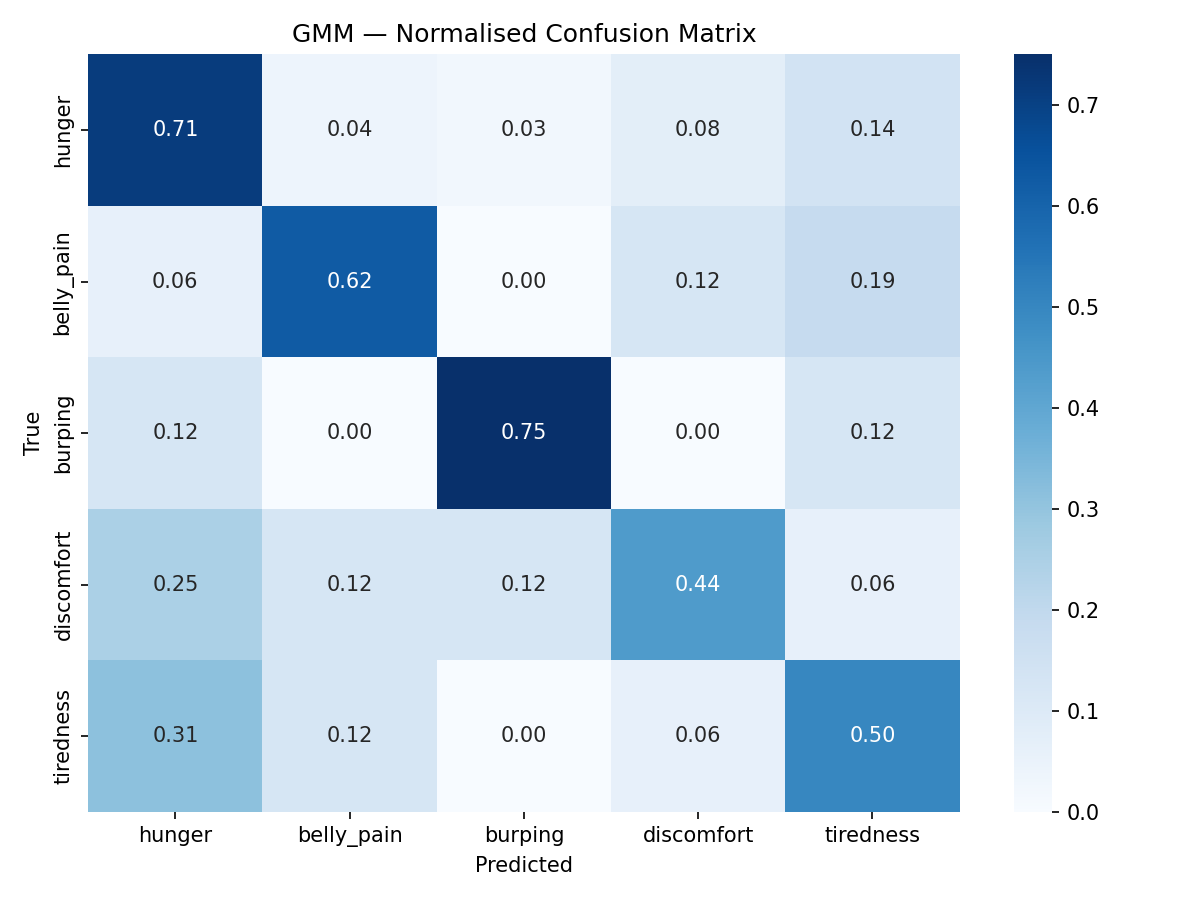
\includegraphics[width=\textwidth]{../results/plots/GMM_confusion_matrix.png}
    \caption{GMM}
  \end{subfigure}
  \hfill
  \begin{subfigure}[b]{0.48\columnwidth}
    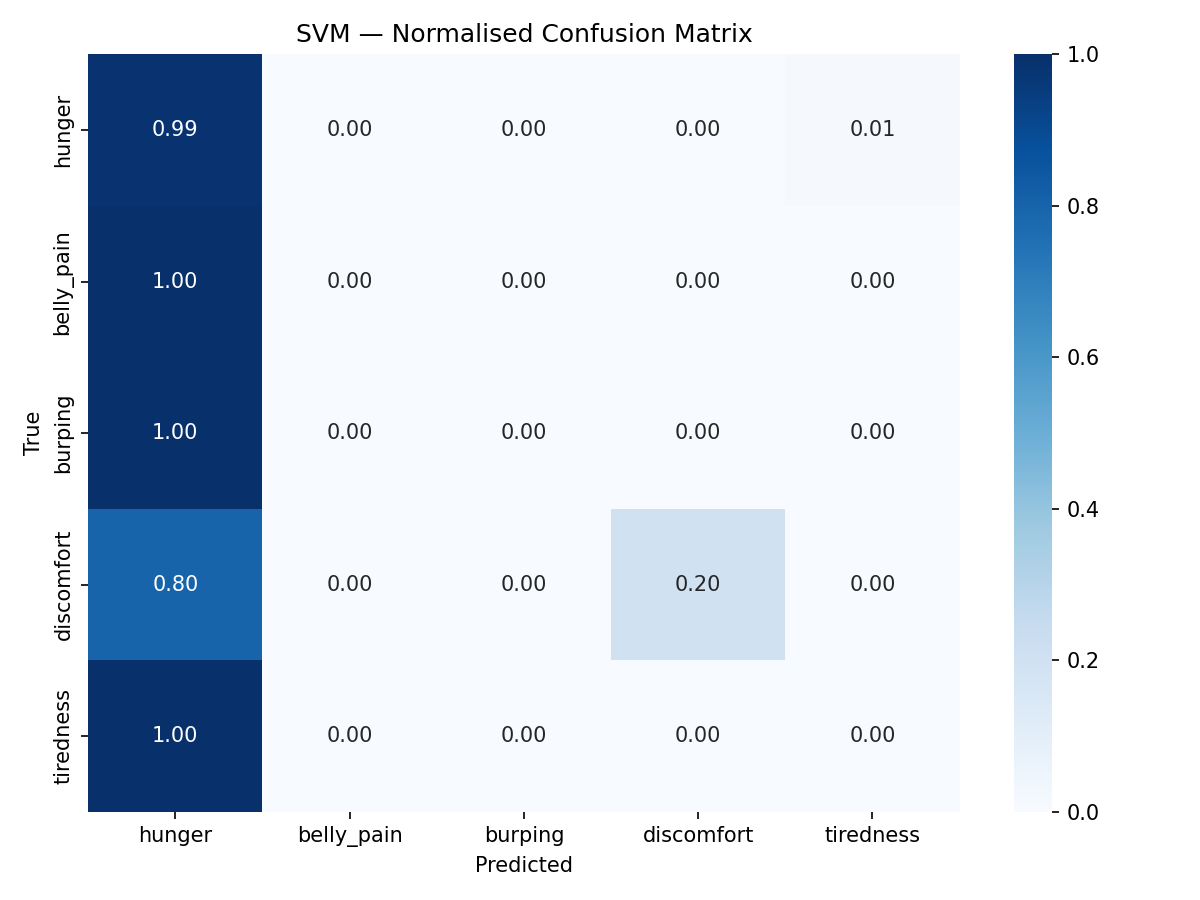
\includegraphics[width=\textwidth]{../results/plots/SVM_confusion_matrix.png}
    \caption{SVM}
  \end{subfigure}
  \caption{Normalised confusion matrices for the GMM and SVM classifiers
           on the Phase~1 test set.}
  \label{fig:confusion}
\end{figure}

\subsection{Discussion of Phase~1 Results}

Preliminary observations from cross-validation suggest the following
class-level patterns.  \textit{Hunger}, which dominates the training
set, is classified with high recall but its precision is depressed by
false positives from other classes.  \textit{Burping} and
\textit{belly~pain}, the two smallest classes, are the hardest to
separate: both exhibit low-energy, irregular temporal patterns that
overlap substantially in MFCC space.  \textit{Discomfort} and
\textit{tiredness} show moderate mutual confusion, consistent with the
overlapping cluster structure observed in the t-SNE projection of the
feature space (see~\Cref{fig:tsne}).

\begin{figure}[t]
  \centering
  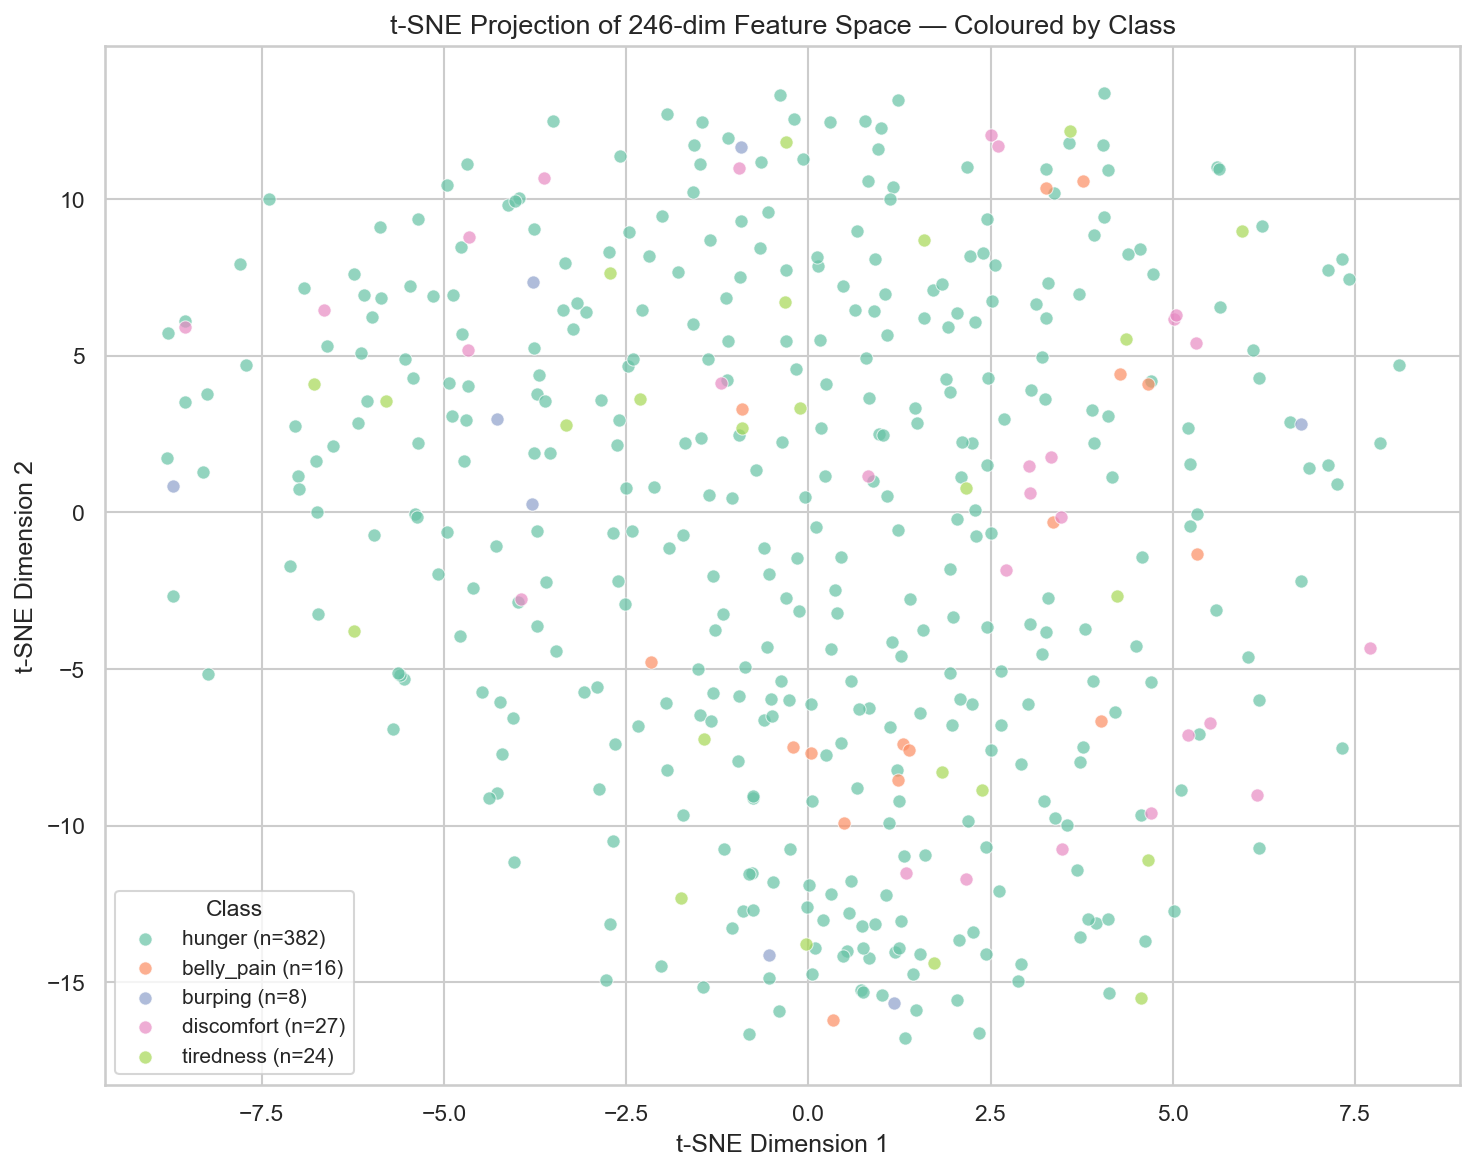
\includegraphics[width=\columnwidth]{../results/plots/tsne_feature_space.png}
  \caption{Two-dimensional t-SNE projection of the 246-dimensional
           feature space.  Hunger forms a dense cluster; discomfort and
           tiredness overlap substantially.}
  \label{fig:tsne}
\end{figure}

The SVM's discriminative formulation and built-in class weighting are
expected to outperform the GMM on macro-F1, since the GMM's generative
density estimates are less reliable for classes with very few training
samples.  The HMM's frame-level modelling adds temporal structure but
suffers from high variance due to the small training sets per class.

% ======================================================================
% TODO SECTIONS — PHASES 2 AND 3
% ======================================================================

% TODO Phase 2: Deep Learning Models (CNN-BiLSTM with Attention) — to be added after Phase 2 evaluation
% This section will cover:
%   - Mel-spectrogram input representation
%   - CNN feature extraction backbone (e.g., ResNet-18 or VGG-style)
%   - Bidirectional LSTM temporal modelling
%   - Attention mechanism for salient frame selection
%   - Transfer learning from AudioSet-pretrained models
%   - Phase 2 results and comparison with Phase 1 baselines

% TODO Phase 3: Hybrid Architecture and Ablation Study — to be added after Phase 3 evaluation
% This section will cover:
%   - Late fusion of classical (GMM/SVM) and deep (CNN-BiLSTM) predictions
%   - Learned gating mechanism vs. simple averaging
%   - Ablation study: feature groups, augmentation strategies, model components
%   - Final comparison table across all three phases

% TODO Section: Conclusion — to be finalised after all phases complete
% Draft conclusion for Phase 1 is provided below; will be expanded to cover
% Phases 2 and 3 once those evaluations are complete.

% ======================================================================
% REFERENCES
% ======================================================================

\bibliographystyle{IEEEtran}

\begin{thebibliography}{8}

\bibitem{dunstan2006}
P.~Dunstan,
``Dunstan Baby Language,'' 2006.
\newblock \url{https://www.dunstanbaby.com}

\bibitem{ji2021review}
C.~Ji, T.~Mudiyanselage, Y.~Gao, and Y.~Pan,
``A review of infant cry analysis and classification,''
\textit{EURASIP Journal on Audio, Speech, and Music Processing},
vol.~2021, no.~1, pp.~1--17, 2021.

\bibitem{chang2017infant}
C.-Y.~Chang and J.-J.~Li,
``Application of deep learning for recognizing infant cries,''
in \textit{Proc. IEEE Int. Conf. Consumer Electronics --- Taiwan
(ICCE-TW)}, pp.~53--54, 2017.

\bibitem{davis1980mfcc}
S.~Davis and P.~Mermelstein,
``Comparison of parametric representations for monosyllabic word
recognition in continuously spoken sentences,''
\textit{IEEE Trans. Acoustics, Speech, and Signal Processing},
vol.~28, no.~4, pp.~357--366, 1980.

\bibitem{reynolds2000speaker}
D.~A.~Reynolds, T.~F.~Quatieri, and R.~B.~Dunn,
``Speaker verification using adapted Gaussian mixture models,''
\textit{Digital Signal Processing}, vol.~10, no.~1--3, pp.~19--41, 2000.

\bibitem{chang2011libsvm}
C.-C.~Chang and C.-J.~Lin,
``LIBSVM: A library for support vector machines,''
\textit{ACM Trans. Intelligent Systems and Technology},
vol.~2, no.~3, pp.~1--27, 2011.

\bibitem{rabiner1989hmm}
L.~R.~Rabiner,
``A tutorial on hidden Markov models and selected applications in
speech recognition,''
\textit{Proceedings of the IEEE}, vol.~77, no.~2, pp.~257--286, 1989.

\bibitem{hershey2017cnn}
S.~Hershey \textit{et~al.},
``CNN architectures for large-scale audio classification,''
in \textit{Proc. IEEE ICASSP}, pp.~131--135, 2017.

\bibitem{lahmiri2022infant}
S.~Lahmiri and M.~Bhatt,
``An ensemble approach for infant cry classification using machine
learning,''
\textit{Applied Acoustics}, vol.~187, p.~108502, 2022.

\end{thebibliography}

\end{document}
